\subsection{SQL Benchmarks}\label{eva: sql_benchmark}
To answer the \textbf{RQ2}, we test the end-to-end performance
of \NAME using the TPC-H benchmarks~\cite{tpc_h} and compare our results
with the corresponding works~\cite{sagma,heda}. Since
SAGMA~\cite{sagma} only uses HE for aggregation, the comparisons are
placed in the Appendix.
% We compare with SAGMA~\cite{sagma}, HEDA~\cite{heda}, and the method of 
% Kortekaa~\cite{aphadb} on the same task
% and evaluate the SQL queries in TPC-H benchmark.
% Moreover, we benchmark a data analysis model (decision tree) based on \NAME.


\begin{figure}[t!]
   \begin{center}
    \begin{subfigure}[b]{0.25\textwidth}
    \centering
    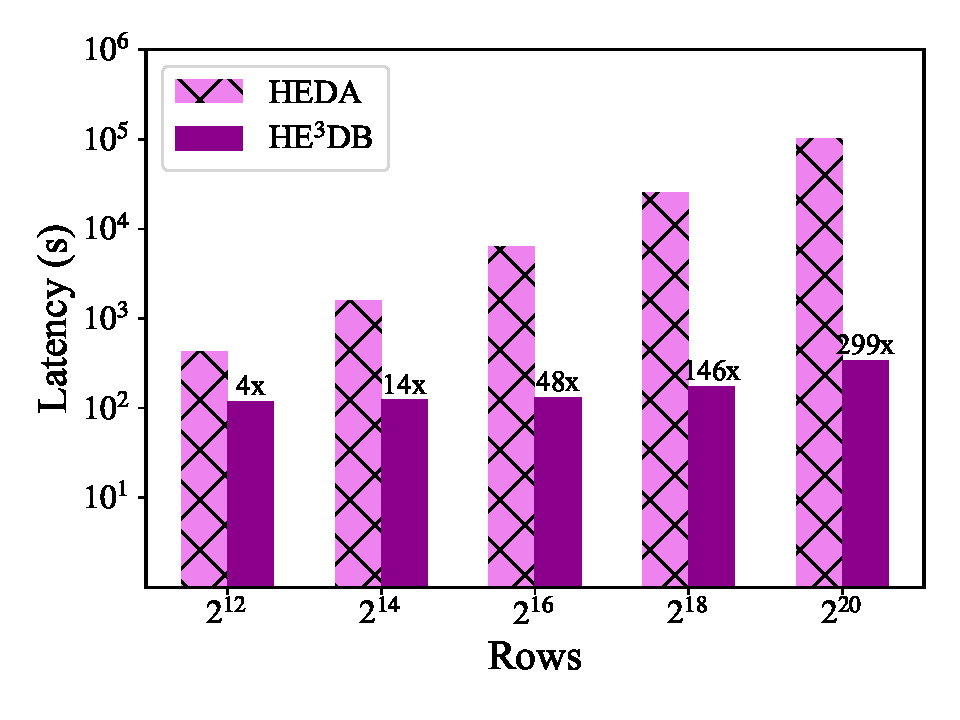
\includegraphics[width=\linewidth]{figure/compare_q1_heda.pdf}
    % \vspace{-1em}
    \caption{Query 1}
    \label{fig: hedaq1}
    \end{subfigure}%
    % \hfill
    \begin{subfigure}[b]{0.25\textwidth}
    \centering
    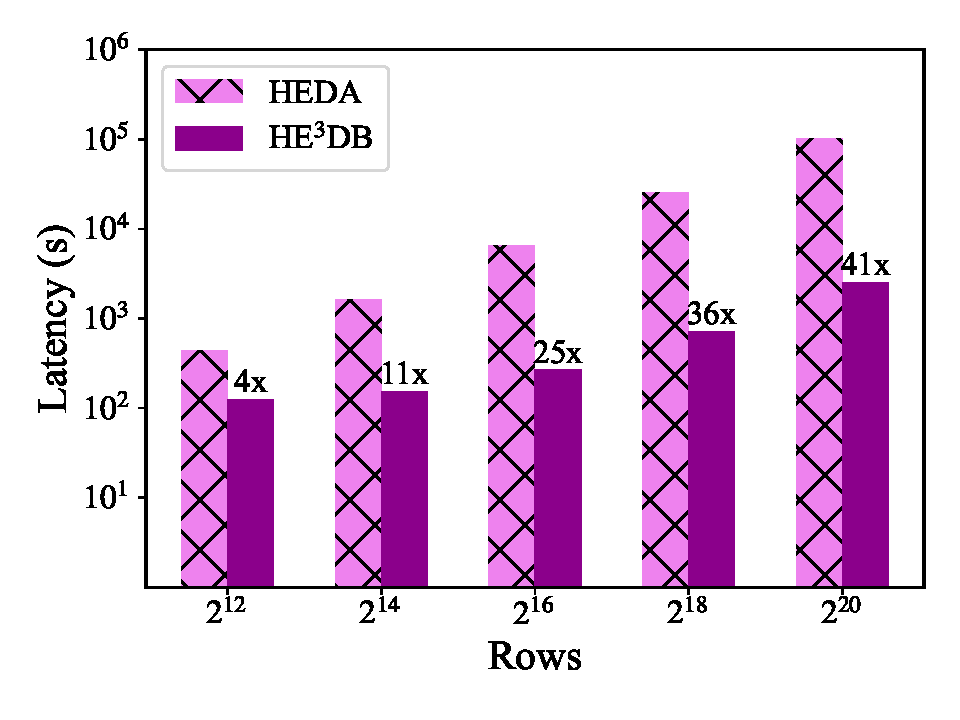
\includegraphics[width=\linewidth]{figure/compare_q6_heda.pdf}
    % \vspace{-1em}
    \caption{Query 6}
    \label{fig: heda16}
    \end{subfigure}%
    % \hfill
   \end{center}
    % \vspace{-1em}
      \caption{Comparison between \NAME and HEDA~\cite{sagma} on their modified TPC-H Query 1 and Query 6 with varying sizes of $\dbtabrow$.} 
      \Description{Comparison between \NAME and HEDA~\cite{sagma} on their modified TPC-H Query 1 and Query 6 with varying sizes of $\dbtabrow$.
      As the size of $\dbtabrows$ increases, 
      the advantage of our performance is more obvious.}
   \label{fig: hedabench}
   % \vspace{-0.5em}
\end{figure}

% {\bf{Aggregation Only}}:
%\paragraph{Aggreagation Only}


\begin{figure}[t!]
   \begin{center}
    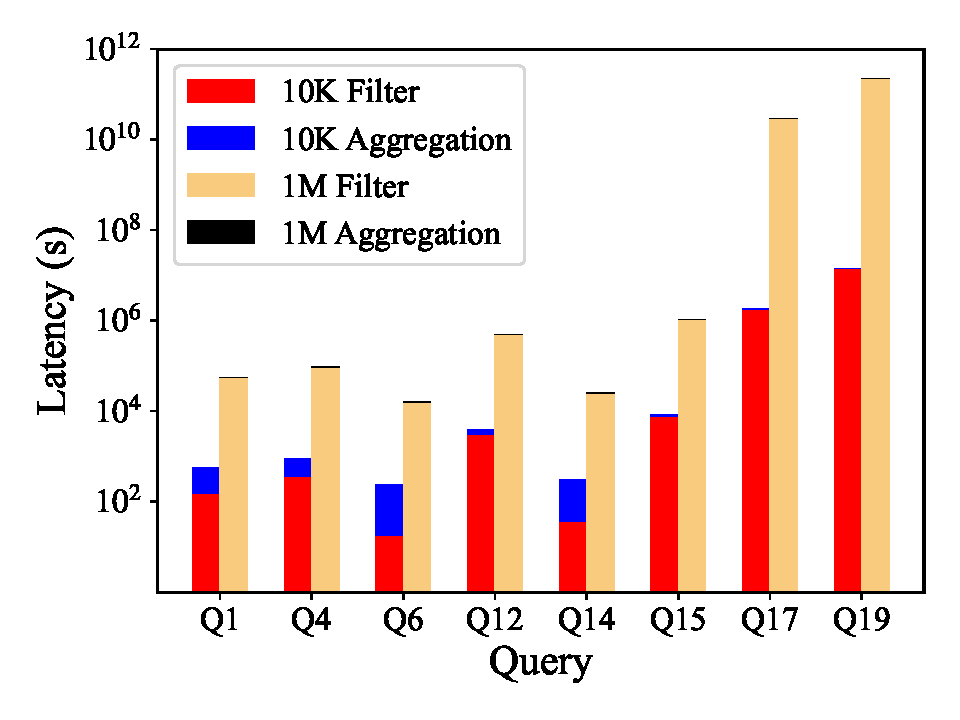
\includegraphics[width=0.9\linewidth]{figure/tpc_h.pdf}
   \end{center}
    % \vspace{-0.5em}
      \caption{Latency performance of \NAME on various TPC-H benchmark
      over different sizes of $\dbtabrow$.} 
      \Description{Latency performance of \NAME on various TPC-H benchmark
      over different sizes of $\dbtabrow$.
      As the size of the database increases, the bottleneck of the entire SQL lies in the filtering period.}
   \label{fig: tpchbench}
   % \vspace{-0.5em}
\end{figure}

% {\bf{TPC-H Benchmarks}}:
%\paragraph{TPC-H Benchmark}
We compare \NAME with HEDA, one of the most recent FHE-based encrypted DBMS
that supports unbounded-depth filter-aggregation~\cite{heda}. As shown in 
\cref{fig: hedabench}, on the same set of TPC-H queries, \NAME 
is on average $299\times$ faster on TPC-H Query 1 and $41\times$ faster on 
TPC-H Query 6. To closely examine the performance breakdown of \NAME,
we test a variety of the TPC-H benchmark queries on our \NAME framework, 
and the results are outlined in \cref{fig: tpchbench}. As the figure shows, while 
the filtering and aggregation latency are somewhat balanced on smaller databases,  
the filtering latency becomes the main performance bottleneck
as the size of the database gets larger. Overall, we can evaluate an end-to-end
SQL query over a 10K-row database within 241 seconds.